\documentclass[%
	11pt,
	a4paper,
	utf8,
	%twocolumn
		]{article}	

\usepackage{style_packages/podvoyskiy_article_extended}


\begin{document}
\title{Заметки по машинному обучению и анализу данных. Том 2}

\author{\itshape Подвойский А.О.}

\date{}
\maketitle

\thispagestyle{fancy}

Здесь приводятся заметки по некоторым вопросам, касающимся машинного обучения, анализа данных, программирования на языках \texttt{Python}, \texttt{R} и прочим сопряженным вопросам так или иначе, затрагивающим работу с данными.


\shorttableofcontents{Краткое содержание}{1}

\tableofcontents

\section{Приемы работы с Catboost}

Онлайн документация пакета \url{https://catboost.ai/en/docs/concepts/python-reference_catboostregressor}.

\subsection{Установка CatBoost}

Установить пакет можно с помощью менеджера \texttt{conda} (или с помощью \texttt{pip})
\begin{lstlisting}[
style = bash,
numbers = none
]
$ conda config --show channels
# если канала conda-forge нет в списке, то следует его добавить 
$ conda config --add channels conda-forge
$ conda install catboost
$ pip install catboost
\end{lstlisting}

\subsection{Ключевые особенности пакета}

\subsection{Параметры}

Ознакомится с описанием параметров можно здесь \url{https://catboost.ai/en/docs/references/training-parameters/}

Общие параметры:
\begin{itemize}
	\item \verb|loss_function| (objective) -- функция потерь, которая используется на шаге обучения модели.
	
	\item \texttt{iterations} -- максимальное число деревьев в ансамбле,
	
	\item \verb*|learning_rate| -- темп обучения,
	
	\item \verb*|l2_leaf_reg| -- коэффициент при члене $ L_2 $-регуляризации,
	
	\item \verb*|bagging_temperature| -- задает настройки Байесовского бутстрапа
\end{itemize}



\subsection{Классификатор CatBoostClassfier}

Класс \texttt{CatBoostClassifier}

\begin{lstlisting}[
style = ironpython,
numbers = none	
]
class CatBoostClassifier(
		iterations=None,
		learning_rate=None,
		depth=None,
		l2_leaf_reg=None,
		model_size_reg=None,
		rsm=None,
		loss_function=None,
		border_count=None,
		feature_border_type=None,
		per_float_feature_quantization=None,                         
		input_borders=None,
		output_borders=None,
		fold_permutation_block=None,
		od_pval=None,
		od_wait=None,
		od_type=None,
		nan_mode=None,
		counter_calc_method=None,
		leaf_estimation_iterations=None,
		leaf_estimation_method=None,
		thread_count=None,
		random_seed=None,
		use_best_model=None,
		verbose=None,
		logging_level=None,
		metric_period=None,
		ctr_leaf_count_limit=None,
		store_all_simple_ctr=None,
		max_ctr_complexity=None,
		has_time=None,
		allow_const_label=None,
		classes_count=None,
		class_weights=None,
		one_hot_max_size=None,
		random_strength=None,
		name=None,
		ignored_features=None,
		train_dir=None,
		custom_loss=None,
		custom_metric=None,
		eval_metric=None,
		bagging_temperature=None,
		save_snapshot=None,
		snapshot_file=None,
		snapshot_interval=None,
		fold_len_multiplier=None,
		used_ram_limit=None,
		gpu_ram_part=None,
		allow_writing_files=None,
		final_ctr_computation_mode=None,
		approx_on_full_history=None,
		boosting_type=None,
		simple_ctr=None,
		combinations_ctr=None,
		per_feature_ctr=None,
		task_type=None,
		device_config=None,
		devices=None,
		bootstrap_type=None,
		subsample=None,
		sampling_unit=None,
		dev_score_calc_obj_block_size=None,
		max_depth=None,
		n_estimators=None,
		num_boost_round=None,
		num_trees=None,
		colsample_bylevel=None,
		random_state=None,
		reg_lambda=None,
		objective=None,
		eta=None,
		max_bin=None,
		scale_pos_weight=None,
		gpu_cat_features_storage=None,
		data_partition=None
		metadata=None,
		early_stopping_rounds=None,
		cat_features=None,
		grow_policy=None,
		min_data_in_leaf=None,
		min_child_samples=None,
		max_leaves=None,
		num_leaves=None,
		score_function=None,
		leaf_estimation_backtracking=None,
		ctr_history_unit=None,
		monotone_constraints=None,
		feature_weights=None,
		penalties_coefficient=None,
		first_feature_use_penalties=None,
		model_shrink_rate=None,
		model_shrink_mode=None,
		langevin=None,
		diffusion_temperature=None,
		posterior_sampling=None,
		boost_from_average=None,
		text_features=None,
		tokenizers=None,
		dictionaries=None,
		feature_calcers=None,
		text_processing=None
)
\end{lstlisting}

LogLoss применяется для задач бинарной классификации (когда целевей вектор содиржит только два уникальных значения или когда параметр \verb|target_border is not None|).

MultiClass используется в задачах мультиклассовой классификации (когда целевой вектор содержит более 2 уникальных значений или параметр \verb|border_count is None|)

\subsection{Регрессор CatBoostRegressor}

Помимо \texttt{iterations} и \texttt{learning\_rate} у CatBoost 5 важнейших гиперпараметров:
\begin{itemize}
	\item \texttt{max\_depth}: мак,
	
	\item \texttt{l2\_leaf\_reg},
	
	\item \texttt{border\_count},
	
	\item \texttt{random\_strength},
	
	\item \texttt{bagging\_temperature}.
\end{itemize}

\subsection{Функции потерь и метрики качества}

\subsubsection{Для классификации}

Для мультиклассификации \url{https://catboost.ai/en/docs/concepts/loss-functions-multiclassification}

\emph{Функции потерь}
\begin{itemize}
	\item LogLoss
\begin{align*}
	- \dfrac{ \sum\limits_{i=1}^N w_i \big( c_i \log p_i + (1 - c_i) \log (1 - p_i) \big) }{ \sum\limits_{i=1}^{N} w_i },
\end{align*}

    \item CrossEntropy
\begin{align*}
	- \dfrac{ \sum\limits_{i=1}^N w_i \big( t_i \log p_i + (1 - t_i) \log (1 - p_i) \big) }{ \sum\limits_{i=1}^{N} w_i },
\end{align*}
\end{itemize}

\emph{Метрики качества}
\begin{itemize}
	\item Precision (точность),
	
	\item Recall (полнота),
	
	\item F1 (гармоническое среднее),
	
	\item BalancedAccuracy
\begin{align*}
	\dfrac{1}{2} \Big( \dfrac{TP}{T} + \dfrac{TN}{N} \Big),
\end{align*}

    \item BalancedErrorRate
\begin{align*}
	\dfrac{1}{2} \Big( \dfrac{FP}{TN + FP} + \dfrac{FN}{FN + TP} \Big),
\end{align*}

    \item AUC,
    
    \item BrierScore,
    
    \item HingeLoss,
    
    \item HammingLoss
\begin{align*}
	\dfrac{ \sum\limits_{i=1}^{N} w_i [[p_i > 0.5] == t_i] }{ \sum\limits_{i=1}^{N} w_i},
\end{align*}

    \item Kappa
\begin{align*}
	1 - \dfrac{1 - Accuracy}{1 - RAccuracy},\\
	RAccuracy = \dfrac{ (TN + FP) (TN + FN) + (FN + TP)(FP + TP) }{ \Big( \sum\limits_{i=1}^{N} w_i \Big)^2 }
\end{align*}

    \item LogLikelihoodOfPrediction.
\end{itemize}

\subsubsection{Для регрессии}

\emph{Метрики качества, которые могут играть роль функции потерь}

\begin{itemize}
	\item MultiRMSE (в случае мультирегрессии)
\begin{align*}
	\Biggl( \dfrac{ \sum\limits_{i=1}^N \sum\limits_{d=1}^{dim} (a_{i,d} - t_{i,d})^2 w_i }{ \sum\limits_{i=1}^N w_i } \Biggr)^{1/2}
\end{align*}
	
	\item MAE
\begin{align*}
	\dfrac{ \sum\limits_{i=1}^{N} w_i | a_i - t_i |}{ \sum\limits_{i=1}^{N} w_i },
\end{align*}

    \item MAPE
\begin{align*}
	\dfrac{ \sum\limits_{i=1}^{N} w_i \dfrac{ | a_i - t_i | }{ \max (1, | t_i |) } }{ \sum\limits_{i=1}^N w_i }
\end{align*}

    \item Poisson
\begin{align*}
	\dfrac{ \sum\limits_{i=1}^N w_i (e^{ a_i } - a_i t_i) }{ \sum\limits_{i=1}^N w_i },
\end{align*}

   \item Quantile (большие значения $ \alpha $ сильнее штрафуют за заниженные прогнозы)
\begin{align*}
	\dfrac{ \sum\limits_{i=1}^N \Big( \alpha - 1[t_i \leqslant a_i] \Big) (t_i - a_i) w_i}{ \sum\limits_{i=1}^N w_i },
\end{align*}

    \item RMSE
\begin{align*}
	\Bigg( \dfrac{ \sum\limits_{i=1}^N (a_i - t_i)^2 w_i }{ \sum\limits_{i=1}^N w_i } \Bigg)^{1/2}
\end{align*}

    \item LogLinQuantile,
    
    \item Lq
\begin{align*}
	\dfrac{\sum\limits_{i=1}^N | a_i - t_i |^q w_i}{ \sum\limits_{i=1}^N w_i }
\end{align*}

    \item Huber
\begin{align*}
	L(t, a) = \sum_{i=0}^N l(t_i, a_i) \cdot w_i,\quad l(t, a) = 
	\begin{cases}
		\dfrac{1}{2} (t - a)^2, &| t - a | \leqslant \delta,\\
		\delta | t - a | - \dfrac{1}{2} \delta^2, &| t - a | > \delta.
	\end{cases}
\end{align*}

\item Excpectile
\begin{align*}
	\dfrac{ \sum\limits_{i=1}^N | \alpha - 1[t_i \leqslant a_i] | (t_i - a_i)^2 w_i }{ \sum\limits_{i=1}^N w_i }
\end{align*}

\item Tweedie
\begin{align*}
	\dfrac{ \sum\limits_{i=1}^N \Big( \dfrac{e^{a_i (2 - \lambda)}}{2 - \lambda} - t_i \dfrac{ e^{a_i ( 1 - \lambda)} }{ 1 - \lambda } \Big) w_i }{ \sum\limits_{i=1}^N w_i },
\end{align*}
где $ \lambda $ -- значение параметра дисперсии мощности,
\end{itemize}

\emph{Метрики качества}

\begin{itemize}
	\item SMAPE
\begin{align*}
	\dfrac{ 100 \sum\limits_{i=1}^N \dfrac{ w_i | a_i - t_i | }{ (|t_i| + |a_i|)/2 } }{ \sum\limits_{i=1}^N w_i }
\end{align*}

    \item R2 (коэффициент детерминации)
\begin{align*}
	1 - \dfrac{ \sum\limits_{i=1}^N w_i (a_i - t_i)^2 }{ \sum\limits_{i=1}^N w_i (\bar{t} - t_i)^2 }.
\end{align*}

    \item MSLE (среднеквадратическая логарифмическая ошибка)
\begin{align*}
	\dfrac{ \sum\limits_{i=1}^N w_i \big( \ln (1 + t_i) - \ln (1 + a_i) \big)^2 }{ \sum\limits_{i=1}^N w_i }
\end{align*}

    \item MedianAbsoluteError
\begin{align*}
	median(|t_1 - a_1|, \ldots, |t_N - a_N|)
\end{align*}
\end{itemize}

\section{Приемы работы с библиотеками Gym и Ecole}

\subsection{Gym}

Функция окружения (environment) \texttt{step} возвращает четыре значения:
\begin{itemize}
	\item \verb|observation| (object):  это объект, специфичный для окружающей среды и представляющий результат наблюдения за этой средой (например, состояние доски в настольной игре),
	
	\item \verb|reward| (float): вознаграждение, полученное за предыдущее действие. Масштаб варьируется в зависимости от среды, но цель всегда в том, чтобы сделать суммарное вознаграждение как можно больше,
	
	\item \verb|done| (boolean): флаг завершения эпизода. Многие (но не все) задачи разделены на четко определенные эпизоды, и \texttt{done = True} указывает на то, что эпизод завершился (например, мы потеряли последнюю жизнь в игре),
	
	\item \verb|info| (dict): диагонстическая информация, полезная для отладки.
\end{itemize}

Это просто реализация классического цикла <<агент -- среда>>. На каждом шаге агент совершает то или иное действие и среда возвращает наблюдения (observation) и вознаграждение (reward).

Процесс запускается вызовом функции \verb|reset()|, которая возвращает первое приближение \texttt{observation}.  
\begin{lstlisting}[
style=ironpython,
numbers=none
]
import gym
env = gym.make('CartPole-v0')
for i_episode in range(20):
    observation = env.reset()
    for t in range(100):
        env.render()
        print(observation)
        action = env.action_space.sample()
        observation, reward, done, info = env.step(action)
        if done:
            print("Episode finished after {} timesteps".format(t+1))
            break
env.close()
\end{lstlisting}

В этом примере мы отбирали случайные действия из пространства действий среды. Каждая среда поставляется с атрибутами \verb|action_space| и \verb|observation_space|. Эти атрибуты имеют тип \verb|Space| и описывают формат допустимых действий и наблюдений
\begin{lstlisting}[
style=ironpython,
numbers=none
]
import gym

env = gym.make("CartPole-v0")
print(env.action_space)  # Discrete(2)

print(env.observation_space)  # Box([-4.8000002e+00 -3.4028235e+38 -4.1887903e-01 -3.4028235e+38], [4.8000002e+00 3.4028235e+38 4.1887903e-01 3.4028235e+38], (4,), float32)
\end{lstlisting}

Пространство \texttt{Descrete} описывает фиксированный диапазон неотрицательных чисел, так что в данном случае допустимыми действиями будет 0 или 1. Пространство \texttt{Box} представляет $ n $-мерный ящик, так что в данном случае допустимыми наблюдениями будут 4-мерные массивы.

\subsection{Ecole}

Полезный ресурс о специальных приемах работы с задачами линейного программирования в частично-целочисленного постановке \url{https://www.gams.com/37/docs/UG_LanguageFeatures.html?search=sos1}

Полезный ресурс по математической оптимизации \url{https://scipbook.readthedocs.io/en/latest/}

\subsubsection{Observations}

Класс \texttt{ecole.observation.NodeBipartiteObs}: двудольный граф наблюдений для узлов branch-and-bound дерева. Оптимизационная задача представляется в виде гетерогенного двудольного графа. Между переменной и ограничением будет существовать ребро, если переменная присутствует в ограничении с ненулевым коэффициентом.

Метод \texttt{reset()} в Ecole принимает в качестве аргумента экземпляр проблемы. 

\section{Отбор признаков с библиотекой BoostARoota}

BoostARoota \url{https://github.com/chasedehan/BoostARoota} -- алгоритм отобора признаков на базе экстримального градиентного бустинга в реализации XGBoost. Алгоритм требует гораздо меньших затрат времени на выполнение. Перед применением необходимо выполнить дамми-кодирование, поскольку базовая модель работает только с количественными признаками.

Отбор признаков выполняется на обучающем поднаборе данных, поэтому предполагается, что массив меток и массив признаков \emph{обучающие}, а для проверки качества модели отбора признаков есть независимая, \emph{тестовая} выборка. Кроме того, если необходимо выбрать оптимальные значения гиперпараметров модели отбора признаков (например, значения гиперпараметров \texttt{cutoff}, \texttt{iters} и \texttt{delta}), то понадобиться еще \emph{проверочная} {выборка}.

\section{HDI}

Highest Density Interval (HDI) -- интервал высокой плотности -- показывает какие точки распределения наиболее достоверны/правдоподобны и охватывают большую часть распределения. Каждая точка внутри интервала имеет более высокую \emph{достоверность}, чем любая точка вне интервала.

\section{Площадь по ROC-кривой}

Построение ROC-кривой происходит следующим образом (\pic{fig:roc_auc0}):
\begin{enumerate}
	\item  Сначала сортируем все наблюдения по убыванию спрогнозированной вероятности положительного класса,
	
	\item Берем единичный квадрат на координатной плоскости. Значения оси абсцисс будут значениями 1 - специфичности (цена деления оси задается значением 1/neg), а значения оси ординат будут значениями чувствительности (цена деления оси задается значением 1/pos). При этом pos — это количество наблюдений положительного класса, а neg — количество наблюдений отрицательного класса,
	
	\item Задаем точку c координатами (0, 0) и для каждого отсортированного наблюдения x:
	\begin{itemize}
		\item если x принадлежит положительному классу, двигаемся на 1/pos вверх,
		
		\item если x принадлежит отрицательному классу, двигаемся на 1/neg вправо.
	\end{itemize}
\end{enumerate}

Значение вероятности положительного класса, при котором ROC-кривая находится на минимальном расстоянии от верхнего левого угла -- точки с координатами (0, 1), дает наибольшую правильность классификации. В данному случае (\pic{fig:roc_auc0-1}) будет 0.72.

\begin{figure}[h]
	\centering
	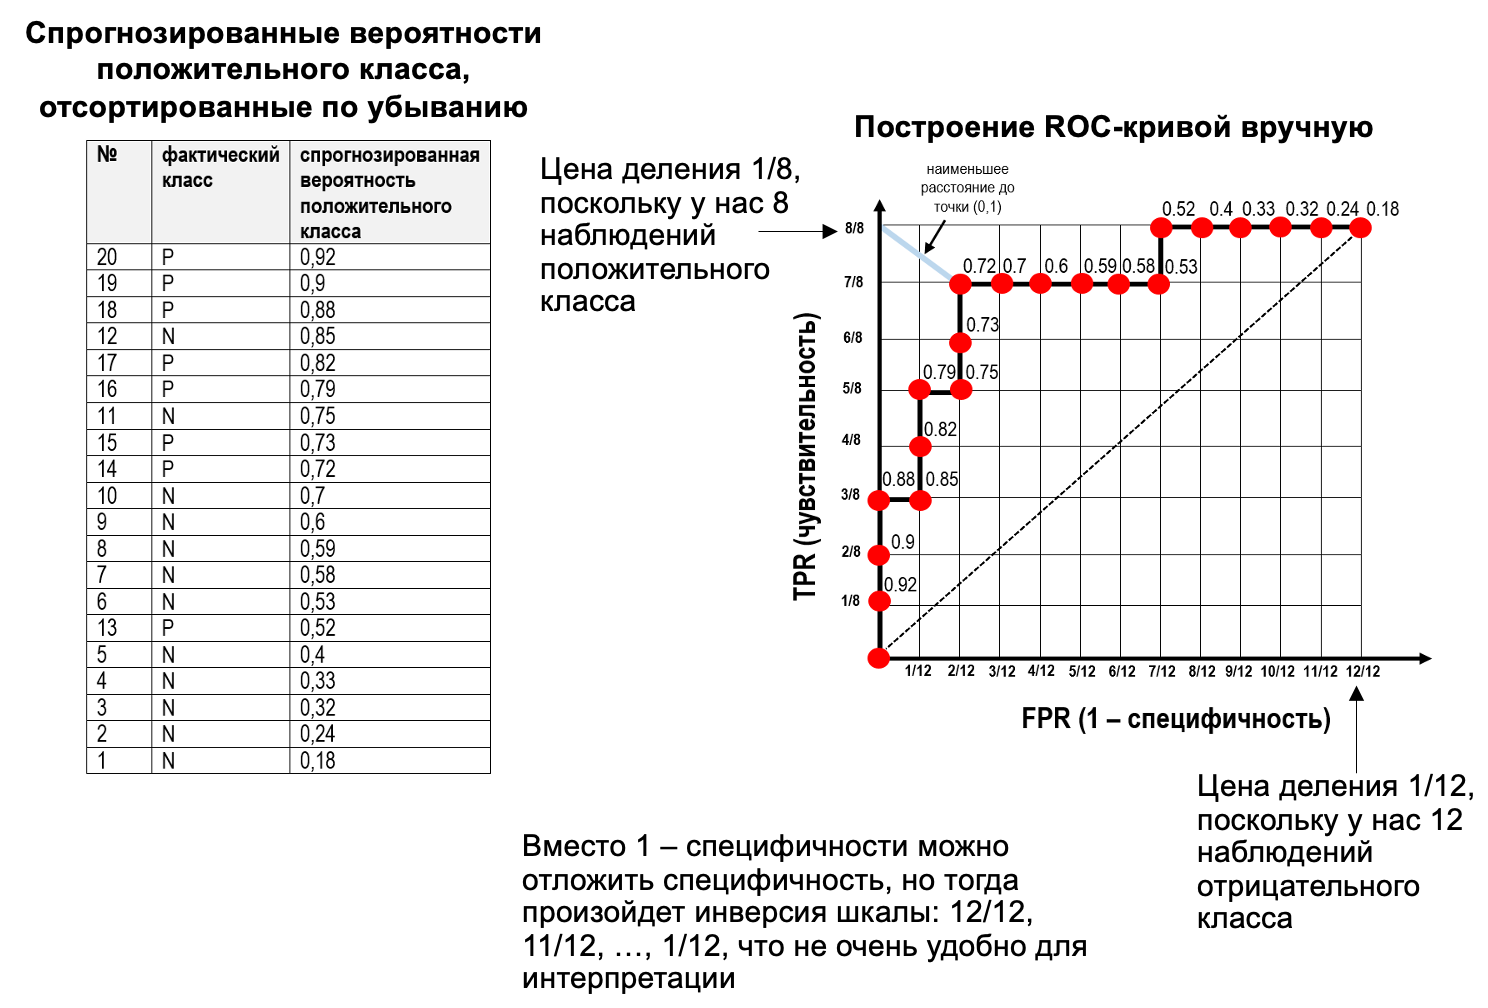
\includegraphics[scale=0.3]{figures/roc_auc0.png}
	\caption{ Построение ROC-кривой }\label{fig:roc_auc0}
\end{figure}

\begin{figure}[h]
	\centering
	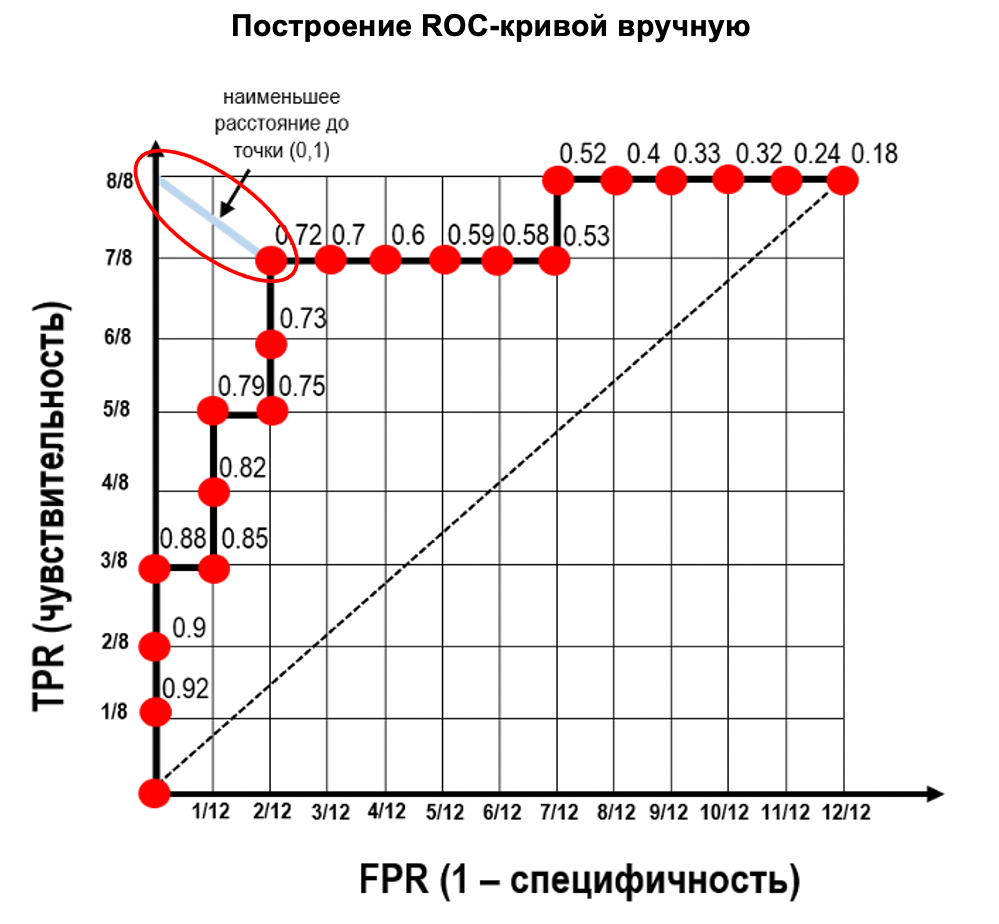
\includegraphics[scale=0.3]{figures/roc_auc0-1.png}
	\caption{ ROC-кривая. Порог отсечения 0.72 }\label{fig:roc_auc0-1}
\end{figure}

Площадь под ROC-кривой (ROC-AUC) можно интерпретировать как вероятность события, состоящего в том, что классификатор присвоит более высокий ранг (например, вероятность) случайно выбранному экземпляру положительного класса, чем случайно выбранному экземпляру отрицательного класса (если не рассматривать вариант равенства значений рангов).

\remark{
На ROC-кривые не влияет баланс классов (при достаточном объеме выборки) и они могут чрезмерно оптимистично оценивать качество работы алгоритма в случае дисбалансов. Лучше пользоваться гармоническим средним или PR-кривыми
}

Однако недостаток такой интепретации заключается в том, что мы пренебрегаем часто встречающейся ситуацией равенства вероятностей. Поэтому правильнее будет сказать, что ROC-AUC равен доле пар вида (экземпляр положительного класса, экземпляр отрицательного класса), которые алгоритм верно упорядочил в соответствии с формулой
\begin{align}\label{eq:rocauc}
	\dfrac{ \sum\limits_{i, j=1}^{n_i, n_j} s(x_i, x_j)}{ n_i \, n_j }, \quad s(x_i, x_j) =
	\begin{cases}
		1, x_i > x_j,\\
		1/2, x_i = x_j,\\
		0, x_i < x_j,
	\end{cases}
\end{align}
где $ x_i $ -- ответ алгоритма для положительного экземпляра, $ x_j $ -- ответ алгоритма для отрицательного экземпляра.

По сути числитель дроби представляет собой сумму количеств $ j $-ых наблюдений отрицательного класса, лежащих ниже каждого $ i $-ого наблюдения положительного класса. Каждое такое количество мы берем по каждому $ i $-ому наблюдению положительного класса в последовательности, отсортированной по мере убывания вероятности положительного класса. Знаменатель дроби -- это произведение количества наблюдений положительного класса и наблюдений отрицательного класса.

Если говорить более точно, мы берем наблюдение положительного класса под номером 20 и каждый раз образовываем пару с наблюдением отрицательного класса (\pic{fig:roc_auc1}), у нас 12 пар, 12 раз наблюдение полжительного класса под номером 20 было проранжировано выше наблюдений отрицательного класса 12, 11, 10 и т.д. Записываем число 12 напротив наблюдения 20. 

Разные модели нельзя сравнивать только по ROC-AUC. ROC-AUC оценивает разные классификатор, используя метрику, которая сама зависит от классификатора. То есть ROC-AUC оценивает разные классификаторы, используя разные метрики.

\remark{
Если часть ROC-кривой лежит ниже диагональной линии, а часть -- выше, то это означает, что классы не являются линейно-сепарабельными, а при этом используется линейная модель
}

При одинаковой ROC-AUC у разных моделей (соответственно с разными ROC-кривыми) будет разное распределение стоимостей ошибочной классификации. Проще говоря, мы можем вычислить ROC-AUC для классификатора A и получить 0.7, а затем вычислить ROC-AUC для второго классификатора и снова получить 0.7, но это не обязательно означает, что у них одна и та же эффективность.

\section{Приемы работы с Gurobi}

Полезный ресурс \url{https://www.gams.com/latest/docs/S_GUROBI.html#GUROBI_GAMS_GUROBI_LOG_FILE}

Чтобы запустить Gurobi в интерактвином режиме, следует в командной оболочке набрать \texttt{gurobi}
\begin{lstlisting}[
title = {\sffamily Сессия GUROBI},
style = bash,
numbers = none
]
gurobi> m = read("./ikp_milp_problem.lp")
gurobi> m.optimize()
gurobi> vars = m.getVars()
gurobi> help(m)
# вывести 2-картежи целочисленных переменных с отличным от нуля значением
gurobi> [(var.varName, var.x) for var in vars if (var.x > 0) and (var.vType == "I")]
gurobi> m.write("res.sol")  # записать решение
\end{lstlisting}


\begin{figure}[h]
	\centering
	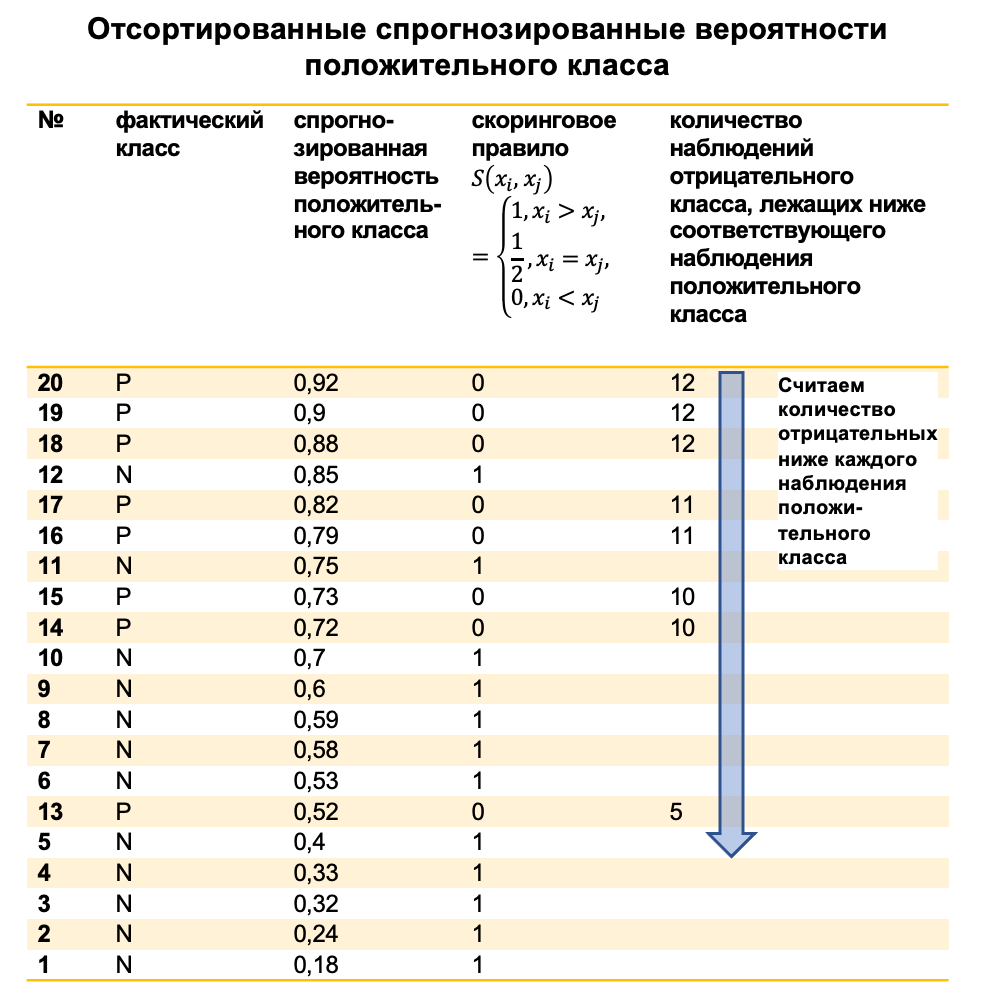
\includegraphics[scale=0.35]{figures/roc_auc1.png}
	\caption{ Расчет ROC-AUC по формуле \eqref{eq:rocauc}}\label{fig:roc_auc1}
\end{figure}

\begin{figure}[h]
	\centering
	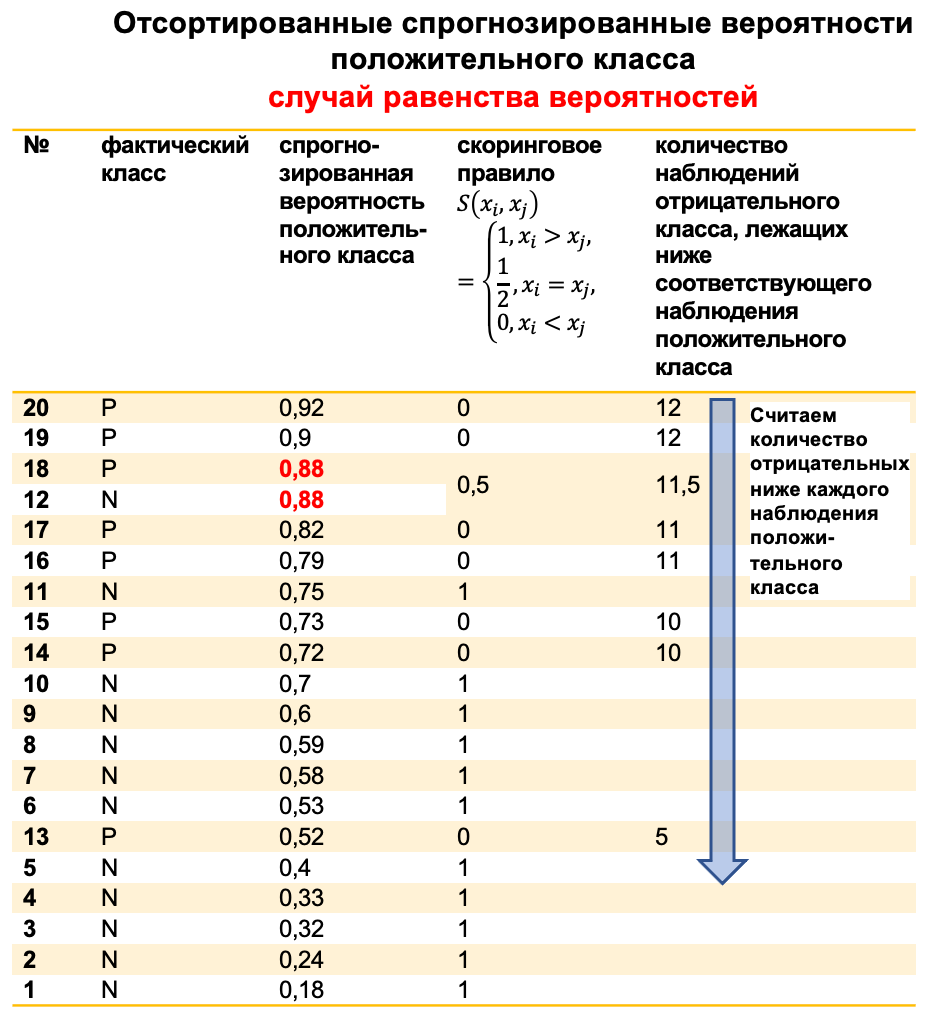
\includegraphics[scale=0.35]{figures/roc_auc2.png}
	\caption{ Расчет ROC-AUC по формуле \eqref{eq:rocauc} для случая равных вероятностей принадлежности экземпляра положительному классу}\label{fig:roc_auc2}
\end{figure}




\listoffigures\addcontentsline{toc}{section}{Список иллюстраций}

% Источники в "Газовой промышленности" нумеруются по мере упоминания 
\begin{thebibliography}{99}\addcontentsline{toc}{section}{Список литературы}
	\bibitem{lutz:learningpython-2011}{\emph{Лутц М.} Изучаем Python, 4-е издание. -- Пер. с англ. -- СПб.: Символ-Плюс, 2011. -- 1280~с. }
		
	\bibitem{beazley:python-2010}{\emph{Бизли Д.} Python. Подробный справочник. -- Пер. с англ. -- СПб.: Символ-Плюс, 2010. -- 864~с. }
\end{thebibliography}

\end{document}
